\documentclass[a4paper]{danarticle}
\usepackage{a4}
\usepackage[pdftex]{color}
\usepackage[pdftex]{graphicx}
\pagestyle{headings}
\usepackage{amsthm}
\usepackage[pdftex,colorlinks=true,
                      pdfstartview=FitB,
                      linkcolor=blue,
                      citecolor=blue,
                      urlcolor=blue,
		      bookmarks=true
          ]{hyperref}
\pdfinfo{
            /Title      (DoorStep: A system for visitor awareness)
            /Author     (Daniel Hahn)
            /Keywords   (Visitors)
}
\newtheorem{definition}{Definition}
\theoremstyle{remark}
\newtheorem*{example}{Example}
\sloppy

\begin{document}
  \author{Daniel Hahn}
  \title{DoorStep: A system for visitor awareness}
  \maketitle
  
  \section{Introduction}
    In recent years, the World Wide Web has become more than just a collection
    of static documents, or even a collection of services. It is now perceived
    as a \textit{social space}, where the \textit{netizens} build virtual
    \textit{places}, \textit{visit} each other and engage in all kinds of
    activities.
    
    It can be assumed that the \textit{hosts} of those places would be
    very interested in what is \lq\lq going on\rq\rq\ in their online
    \textit{territory} --- if
    there was a convenient way of monitoring the activity. 
    
    Although
    information about the \textit{visits} is readily available in the
    form of web server logs, the usual tools for displaying it (e.g. 
    AWStats\cite{awstats}) will only
    provide statistical information but do not explore the rich context in which
    the visits took place. 
    
    Initial research into the subject by Gellersen and Schmidt\cite{webaware}
    yielded the
    \textit{glances into visitor's sites} approach. They assumed that most of
    the visitors to a site had their own place somewhere on the web, and that
    presenting those places to the host would give him an understanding of the
    kind of \textit{territory} his or her place is in.
    
    In this paper we will take this approach a step further: We will argue that
    even if the visitor does not have an own place (or if we are
    simply unable to find it) she will always have \textit{relations} to various
    places, and in following different types of relations we may be able to
    explore different types of \textit{territories} that in some way adjacent to
    the host's place.
    
    The notion of \emph{relations} between web places is not an entirely new 
    one: Relations by hyperlinks and web communities have already 
    been the subect of research by Flake\cite{flake}, Gibson\cite{gibson}, 
    Larson\cite{larson} and others. 
    Adamic and Adar\cite{links}, for example, not only found 
    evidence that a hyperlink indicates a social relation, but also that 
    clusters of hyperlinked pages indicate social groups that can be identified 
    with relative ease. These findings are important for the current work, 
    since they prove the way of exploring relations is a viable one. The main
    interest of this work, however, was to show that meaningful relations 
    between pages exists and to identify groups of related pages. The
    researchers do not suggest in which particular way their findings should be 
    applied or presented to the end user. 
    The DoorStep system, on the other hand, is based on the assumption that 
    meaningful relations between web places do exist but does not concern itself 
    with the exact nature of those relations -- in fact, the system is designed 
    to work with almost all imaginable kinds of relations. What we propose is an 
    efficient way to exploit exisiting relations, connect them to visit events 
    and prepare the results in way that makes it easy to present them to an end 
    user.
    
    Again, the DoorStep system itself does not concern itself with the exact 
    nature of the end user display. And while we propose the use of an ambient 
    display (like proposed in \cite{ambient}), the system allows for many 
    different ways of displaying the results.
    
    We will introduce a system for finding places that are \textit{related} to
    visitors and will present the results which we gathered from a first
    implementation of this system.
  \section{The DoorStep System}
    DoorStep is a system that attempts to find \textit{places} which are somehow
    \textit{related} to \textit{visits}. We assume that each
    of this \textit{places} can be described by an URL of the form described in
    \cite{url}. Furthermore, we will use the naming conventions and definitions
    introduced in \cite{webaware}:
    \begin{center}
    \begin{minipage}{10cm}
    \itshape
    In the web infrastructure, a web place [\dots] is defined as 
    a set of resources in the web. Resources can
    be HTML documents, images, other media objects or arbitrary applications.
    These resources are made available by web servers, i.e. programs that manage
    resources and make them available worldwide through the web protocols. A
    visit to a web place then relates to a request for a resource in the
    designated set. A request originates from a client, i.e. a program the
    visitor uses to specify his request, typically a standard web browser. Web
    servers routinely log requests for resources [\dots]. These server logs
    constitute a rich source on web activity.
    \end{minipage}
    \end{center}
    There are documents (such as \cite{logfile}) that describe in great detail 
    the data available from web server log files. The most important fields used 
    in the DoorStep system are:
    \\
    
    \textbf{Client Address:} The network address of the client system to which 
    the requested resources are sent. This is either the IP address of the 
    computer which is running the visitor's web browser or, if http proxies are 
    involved, the address of a proxy server. We will also call this the 
    \textbf{visit source}
    \\
    
    \textbf{Timestamp:} The date and time at which the request was recieved.
    \\
    
    \textbf{Resource:} A description of the resource that was requested.
    \\
    
    \textbf{User Agent:} A string identifiying the visitor's user agent 
    software. This usually consists of the name and version of the browser, 
    crawler or toolkit that was used make the connection.
    \\
    
    \textbf{Referer:} An URL describing the resource which referred to the local 
    resource. (e.g. the URL of the page that contained the hyperlink to the 
    local page).
    \\
    
    Additionally to
    this \textit{primary} information, data may be gathered from the
    context of the visit: For example, a certain \verb$User-Agent$ header 
    may indicate a certain type of visitor (e.g. a crawler or bot), or a visit
    from a visitor in the \verb$.co.uk$ domain can be assumed to come from
    Britain. Both the primary and secondary information may be used for finding
    relationships.
    \subsection{System overview}
      When the system recieves a visit, it will first attempt to find one or 
      more URLs that act as starting points for further processing. These 
      starting points should have a close connection to the original visit since 
      they will represent it during the following steps.
      
      The starting points will then be fed into a network of \textit{relation 
      finders} that attempt find URLs of web places that are somehow related to 
      the them. The \textit{relation finder} network is the central part of the 
      system: It follows the implicit and explicit connections that link one 
      place with it's neighbours and thus explores the virtual surroundings of 
      the starting point. 
      
      \begin{figure}[ht]
        \centering
        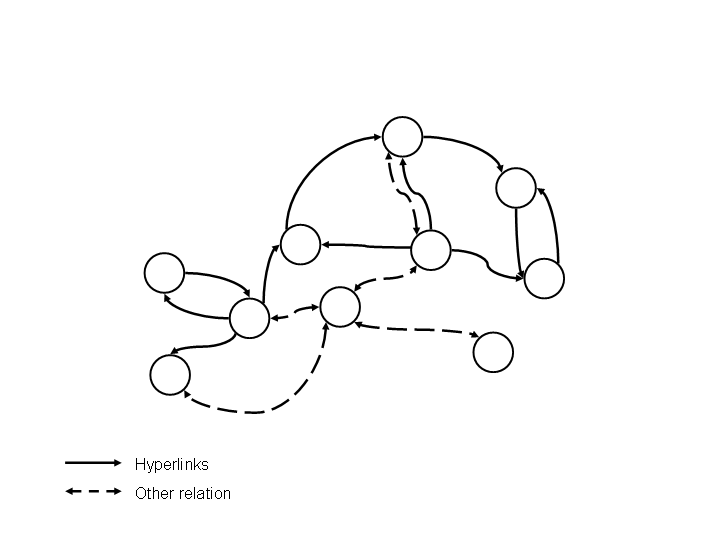
\includegraphics[width=10cm]{webgraph}
        \caption{The web as a graph}
        \label{webgraph}
      \end{figure}
      The relation finding step treats the whole network as a huge graph, of
      which the web places (and other machines) are the vertices. A relation
      between two web places can then be thought of as an edge of the graph,
      connecting those places. Relations can either be directed, like
      hyperlinks, or undirected. The relation finder will enter the graph at the
      starting vertices found in the first step and from there explores paths to
      neighbouring vertices.
      
      At the end of the relation finding phase, the system will have found a
      cluster of web places, representing the virtual neighbourhood of the
      visitor. Each of them will be rated by a number of \textit{rating
      functions} in order to determine how interesting they may be to the user.
      The rated places will then be passed on to a display system that presents
      them to the user.
      \begin{figure}[ht]
        \centering
	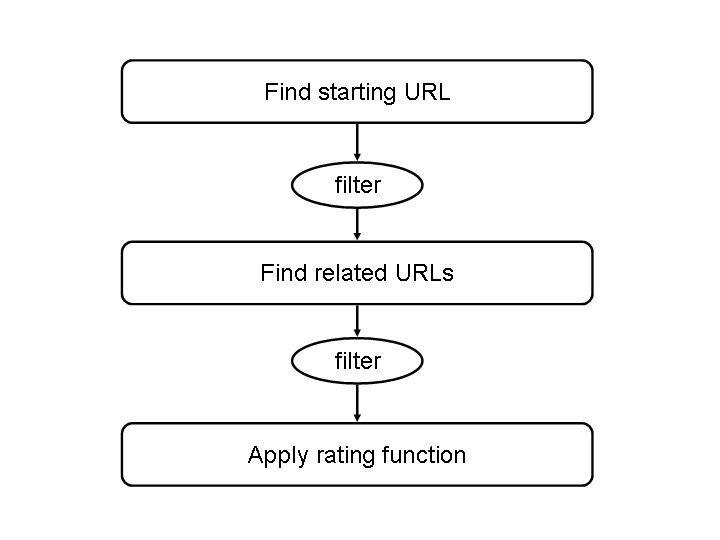
\includegraphics[width=10cm]{steps_overview}
	\caption{Major processing steps of DoorStep}
	\label{steps_overview}
      \end{figure}
    \subsection{Finding starting places}
       \begin{figure}[ht]
       \centering
	 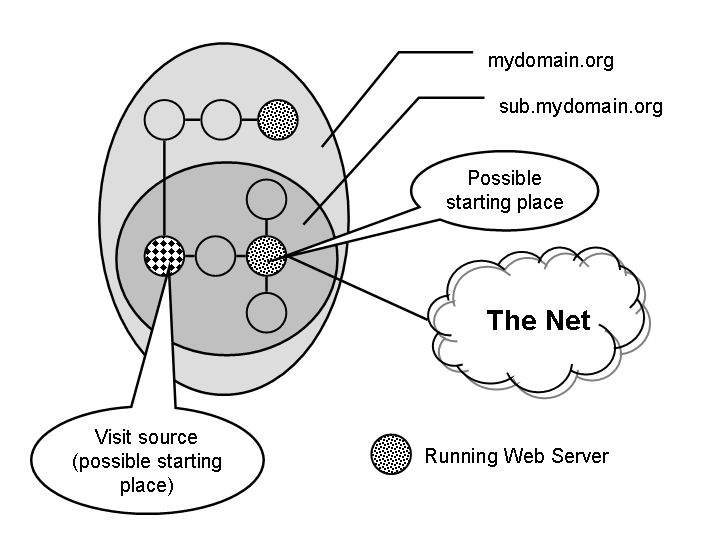
\includegraphics[width=10cm]{startingplace}
	 \caption{Selecting a starting place}
	 \label{startingplace}
       \end{figure}
       Relations between web places are easy to describe and handle. Relations
       between visits, visitors and places, however, are somewhat harder to
       grasp. To avoid the complications of modeling those relations the system
       will pick one (or several) web places that act representatives, or
       proxies, for the visit. These are the \textit{starting places} of the 
       relation finding process,
       in the graph model these are the nodes from which the algorithm will
       start exploring the edges. 
       
       Each starting point must have a close connection to the visit that it is
       ment to represent. In terms of the DoorStep system we demand that a
       starting point should be \textit{as close as possible} to the visit it is
       representing. The metric that measures the \lq\lq distance\rq\rq\ between
       a visit and a web place will vary depending on the type of visit and the
       information at hand, but for HTTP visits (that originate from a network
       address) we use the following
       \begin{definition}
       \label{metric}
       The distance between two hosts with the fully qualified DNS host names
       \verb$a_part[n].a_part[n-1]. ... .a_part[0]$ and 
       \verb$b_part[m].b_part[m-1]. ... .b_part[0]$ of the format given in
       \cite{dns} and with the subdomain tokens \verb$a_part[]$ and 
       \verb$b_part[]$ is given by the number of matching right-hand tokens.
       \end{definition}
       A similiar metric can easily be construed for hosts that have no
       qualified DNS name but only a network address, although we found that
       most of the visit source do have a qualified hostname and those that do
       not weren't particularly useful either.
       
       With the metric from Definition \ref{metric}, the hostname closest to a
       visit source is always that of visit source itself. In most cases,
       however, this host is not really web place because there is no web server
       running at that address -- we say that the respective URL is not
       \textit{alive}. Having starting points that are not \textit{alive} can
       be somewhat awkward during the relation finding phase (e.g. if trying to
       follow the hyperlinks from the starting points), and in these cases we
       will attempt to find \textit{alive} starting points using the algorithm
       already used in \cite{webaware}:
       
       \begin{itemize}
         \item{If the visit source is, copy it to the output}
	 \item{As long as the hostname has more than two tokens, do the
	 following:}
	 \begin{itemize}
	   \item{Try if the new hostname, prefixed with \verb$www$ is alive.}
	   \item{If it is alive, copy it to the output.}
	   \item{Remove the first token from the hostname.}
	 \end{itemize}
       \end{itemize}
       
       For example, if a visit comes from the host
       \verb$banana.hoogla.boogla.org$, the algorithm would first try that
       host itself (Distance 0), then \verb$www.hoogla.boogla.org$ (Distance 1),
       then \verb$www.hoogla.boogla.org$ (Distance 2) and finally
       \verb$www.boogla.org$ (Distance 3). If any of those hosts is
       \textit{alive} it may be used as a starting point. If that is not the
       case, the algorithm fails.
       \begin{figure}[ht]
       {\ttfamily
       \begin{tabbing}
           \hspace{5mm} \= \hspace{5mm} \= \hspace{5mm} \= \hspace{5mm} \= \\
	   @subdom\_parts = \textit{split}(\verb$/\./$, visit\_source); \\
	   \\
	   \textbf{if} ( \textit{\&alive}(join(\verb$'.'$, @subdom\_parts) \{
	   print OUT @subdom\_parts; \} \\
	   \textbf{for} \verb-( ; $#parts > 0 ; shift(@parts) )- \{ \\
	   \>  \textbf{if} ( \textit{\&alive}("www." . join(\verb$'.'$,
    	   @subdom\_parts))) \{ \\
	   \> \> print OUT www . @subdom\_parts; \\
	   \> \} \\
	   \} \\
         \end{tabbing}}
	 \caption{Algorithm for selecting alive starting points}
	 \label{domaintest}
       \end{figure}
     \subsection{Finding related places} 
       A network of \textit{relation finders} is the central processing unit of 
       the DoorStep system. A \textit{relation} finder is an object that will 
       examine a web place (an URL) and attemps to find other URLs that are 
       related to it. In the following definitions, the term \lq\lq URL\rq\rq\ 
       is used as a convenient shorthand for \lq\lq web place\rq\rq . However, 
       these URL objects do not only contain the resource locator as described 
       in \cite{url}, but \emph{all} information the system has gathered about 
       the web place addressed by that locator. This includes both information 
       about  the resources served from that URL (e.g. document type, hyperlinks) 
       and information retained from the original visit event (if the URL is a 
       starting point).
       \begin{definition}
       An URLs $ u_1 $ is related to another URL $ u_2 $ by some relation 
       $ \rightarrow $
       ($ u_1 \rightarrow u_2 $) if it has some characteristic $ c $ in regard
       to $ u_2 $. The characteristic can usually described by a boolean
       relationship function: $ c = r_{\rightarrow}(u_1, u_2) $:
       \[
         r_{\rightarrow}(u_1, u_2) = \hspace{1mm} \mbox{true} \hspace{2mm} 
	     \Leftrightarrow \hspace{1mm} u_1 \rightarrow u_2
       \]
       $ U_{\rightarrow}(u_x) $ is the set of all URLs that a given URL $ u_x $ 
       is related to (by the relation $ \rightarrow $), and it's members are 
       called the \emph{relatives} of $ u_x $.
       \end{definition}
       In the graph model of the network, this kind of relation is equivalent
       with a directed edge from $ u_1 $ to $ u_2 $, and we say that $ u_1 $ is
       \textit{weakly related} to $ u_2 $. \textit{Strong relations} are
       equivalent to undirected edges.
       Examples of relations include hyperlinks (weak) or web places that are
       within the same DNS domain (strong). 
       \begin{definition}
       Two URLs $ u_1 $ and $ u_2 $ are \emph{strongly related} by a relationship
       $ \rightarrow $ if $ u_1 \rightarrow u_2 $ as well as 
       $ u_2 \rightarrow u_1 $. A relationship $ \leftrightarrow $ is called a
       \emph{strong} relationship if
       \[
         u_1 \leftrightarrow u_2 \Rightarrow u_2 \leftrightarrow u_1 
       \]
       for all possible URLs $ u_1 $ and $ u_2 $. In the case of a strong 
       relationship, $ U_{\leftrightarrow}(u_x) $ will be an equivalency 
       class, and $ \leftrightarrow $ an equivalency relation.
       \end{definition}

       When a relation finder $ F $ examines an URL $ u_x $, it will attempt to 
       find a set of URLs to which $ u_x $ is related by some relation 
       $ \rightarrow_F $. It isn't neccessary that the relation finder finds 
       \emph{all} relatives of $ u_x $, a subset of $ U_{\rightarrow_F}(u_x) $ 
       will suffice. In practice, the relation finder will only be able to find 
       all relatives if $ U_{\rightarrow_F}(u_x) $ can be computed from $ u_x $ 
       without further knowledge (i.e. if $ u_x \rightarrow_F u_y $ means 
       $ u_x $ contains a hyperlink to $ u_y $ then $ u_x $ contains all 
       information to compute $ U_{rightarrow_F}(u_x) $). In all other cases the 
       relation finder will contain a heuristic that selects a set of 
       \textit{candidate} URLs that are possibly related to $ u_x $. From these 
       candidates it will then select the relatives of $ u_x $. In practice the 
       heuristic will often include the use of a web search engine like 
       \cite{google}. Those engines have several properties that make the well 
       suited for relation finded an will be discussed in detail in the next 
       section.
       \begin{figure}[ht]
         \centering
	     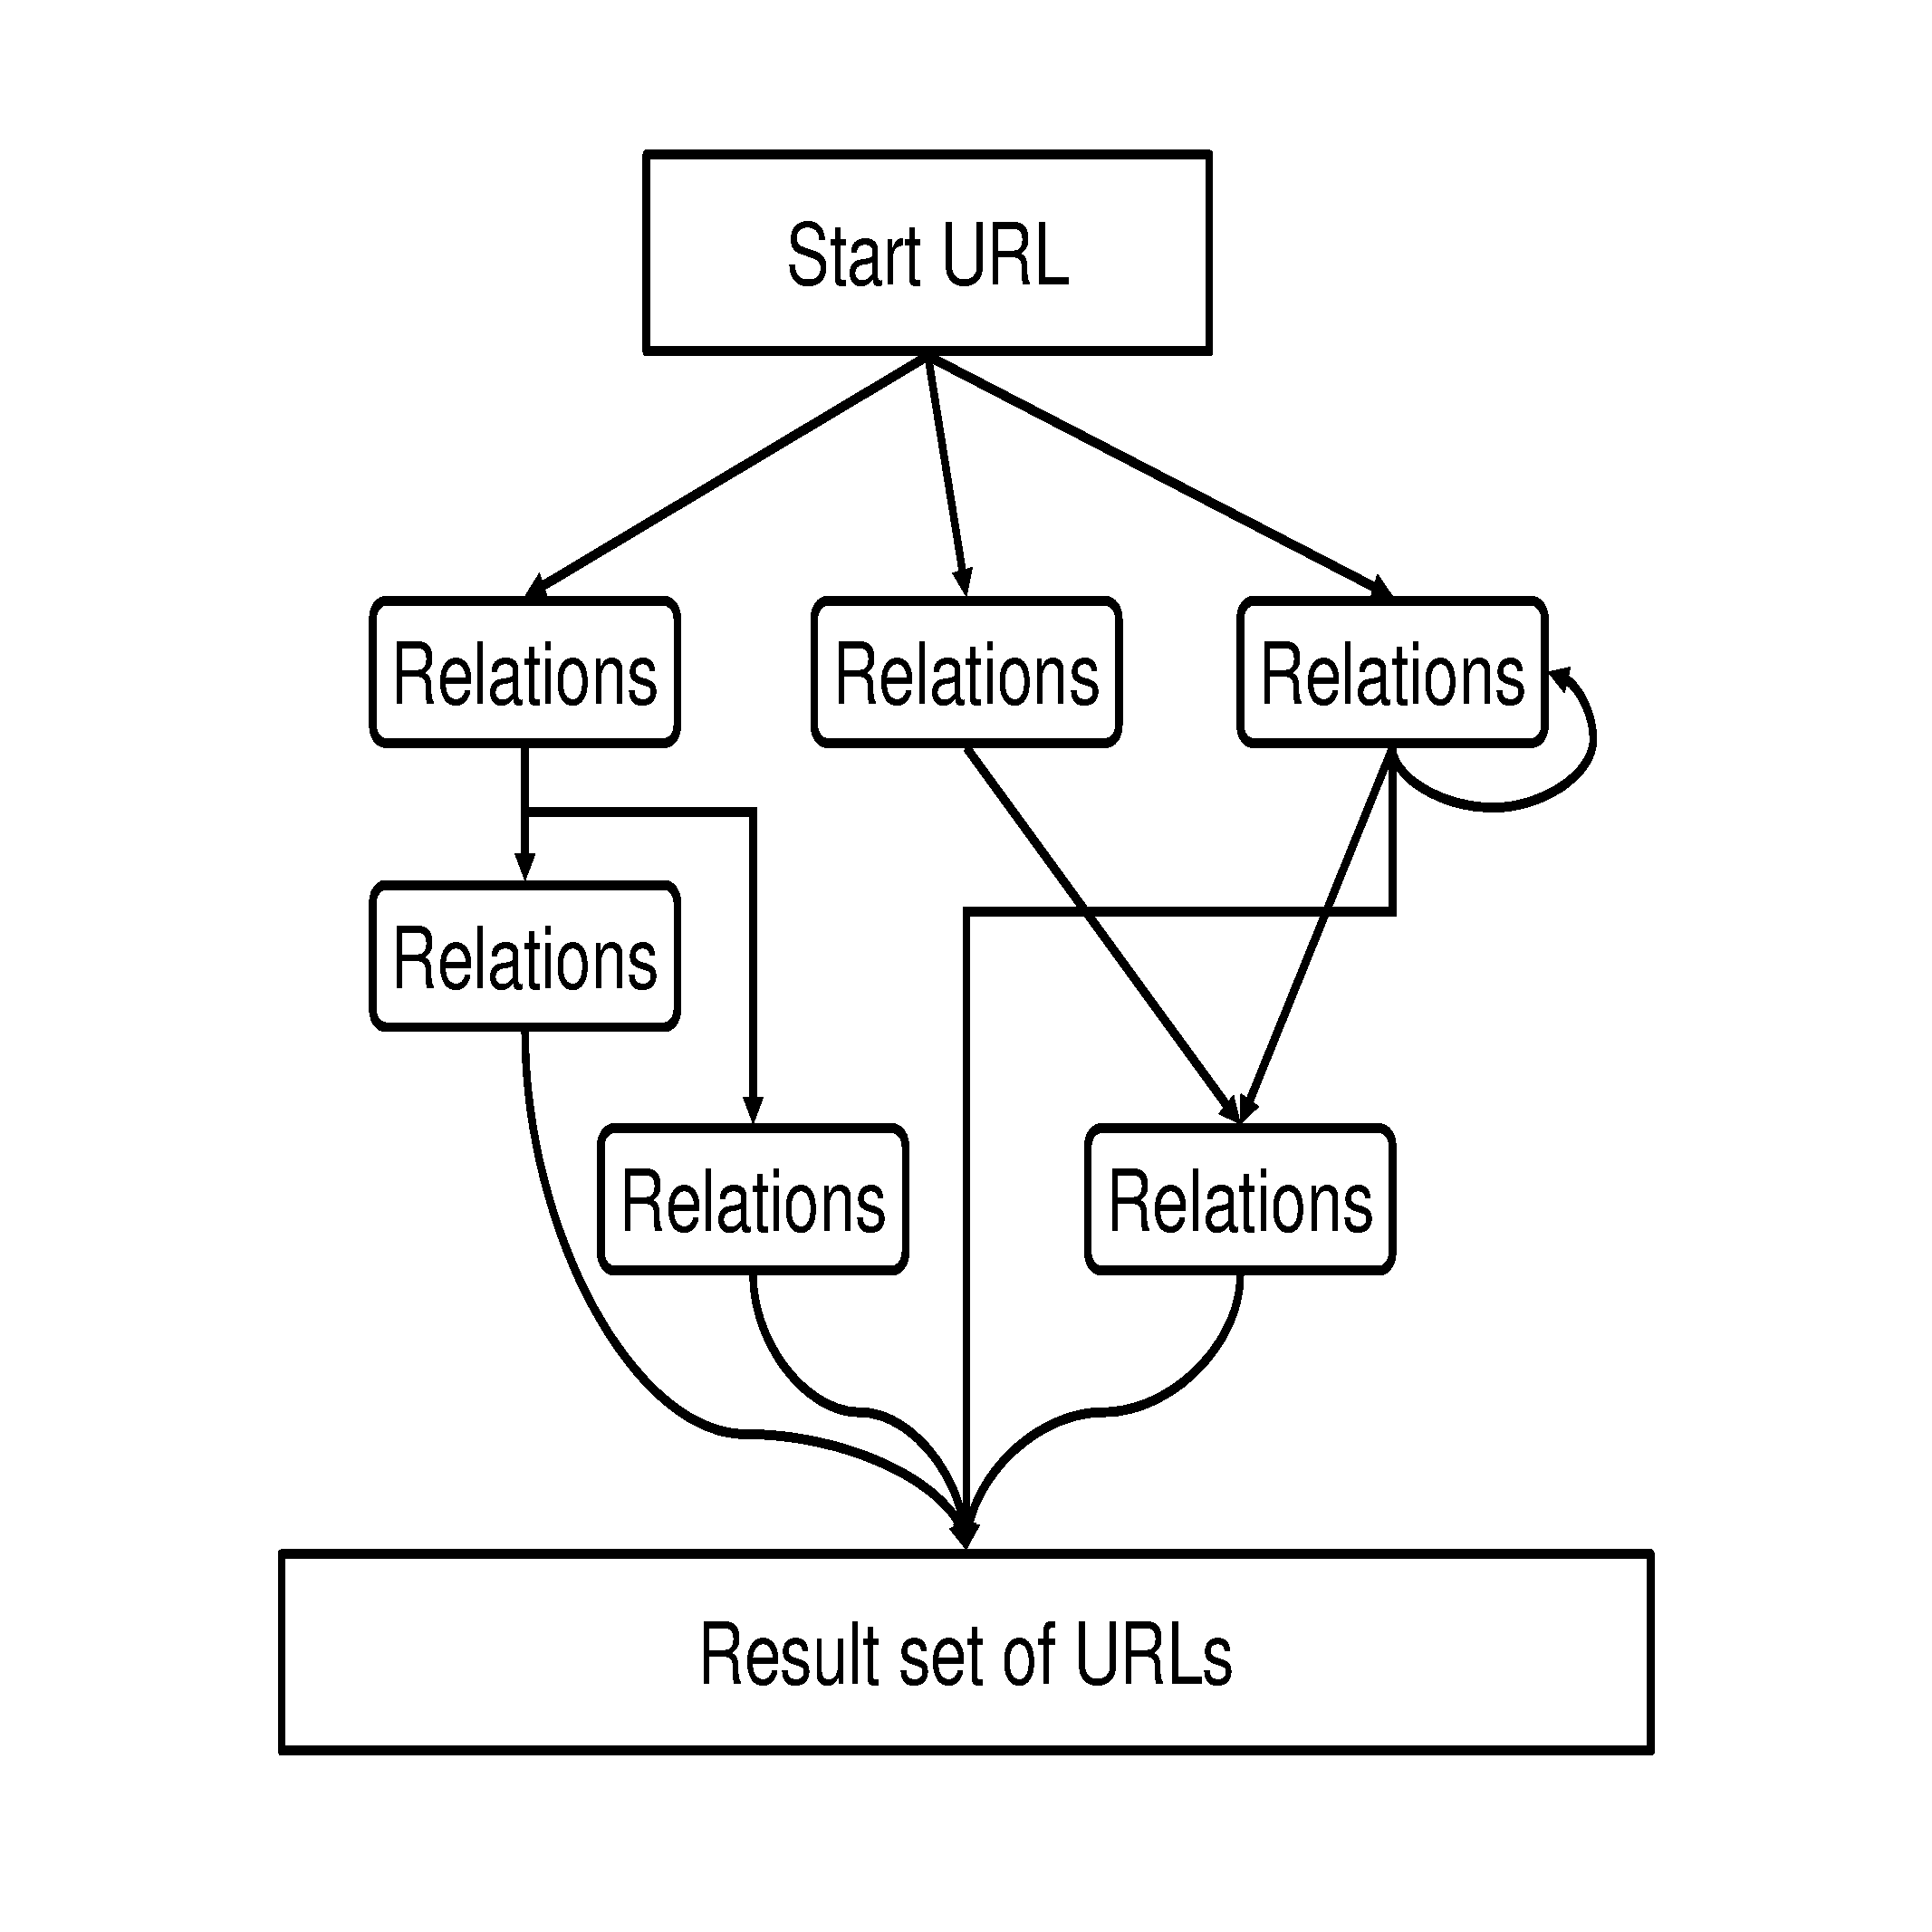
\includegraphics[width=10cm]{relations}
	     \caption{Data flow through different relation finder instances}
	     \label{relations}
       \end{figure}
       The relation finders are arranged in a network structure like shown in 
       Figure \ref{relations}. A relation finder reads a set of URLs from it's 
       input and finds related URLs for each of them. The relation 
       finder then passes the result set either to the output of the relation 
       finding phase or to the input of one or more relation finders (including 
       itself).
       
       In the graph model, a relation finder will work on a single node at a 
       time, attempting to find edges that go from the original node to 
       neighbouring ones. The nodes that are found in this way may then then be 
       used as starting points for further relation finders.
     \subsection{Degrees of relationship}
       \begin{figure}[ht]
       \centering
	 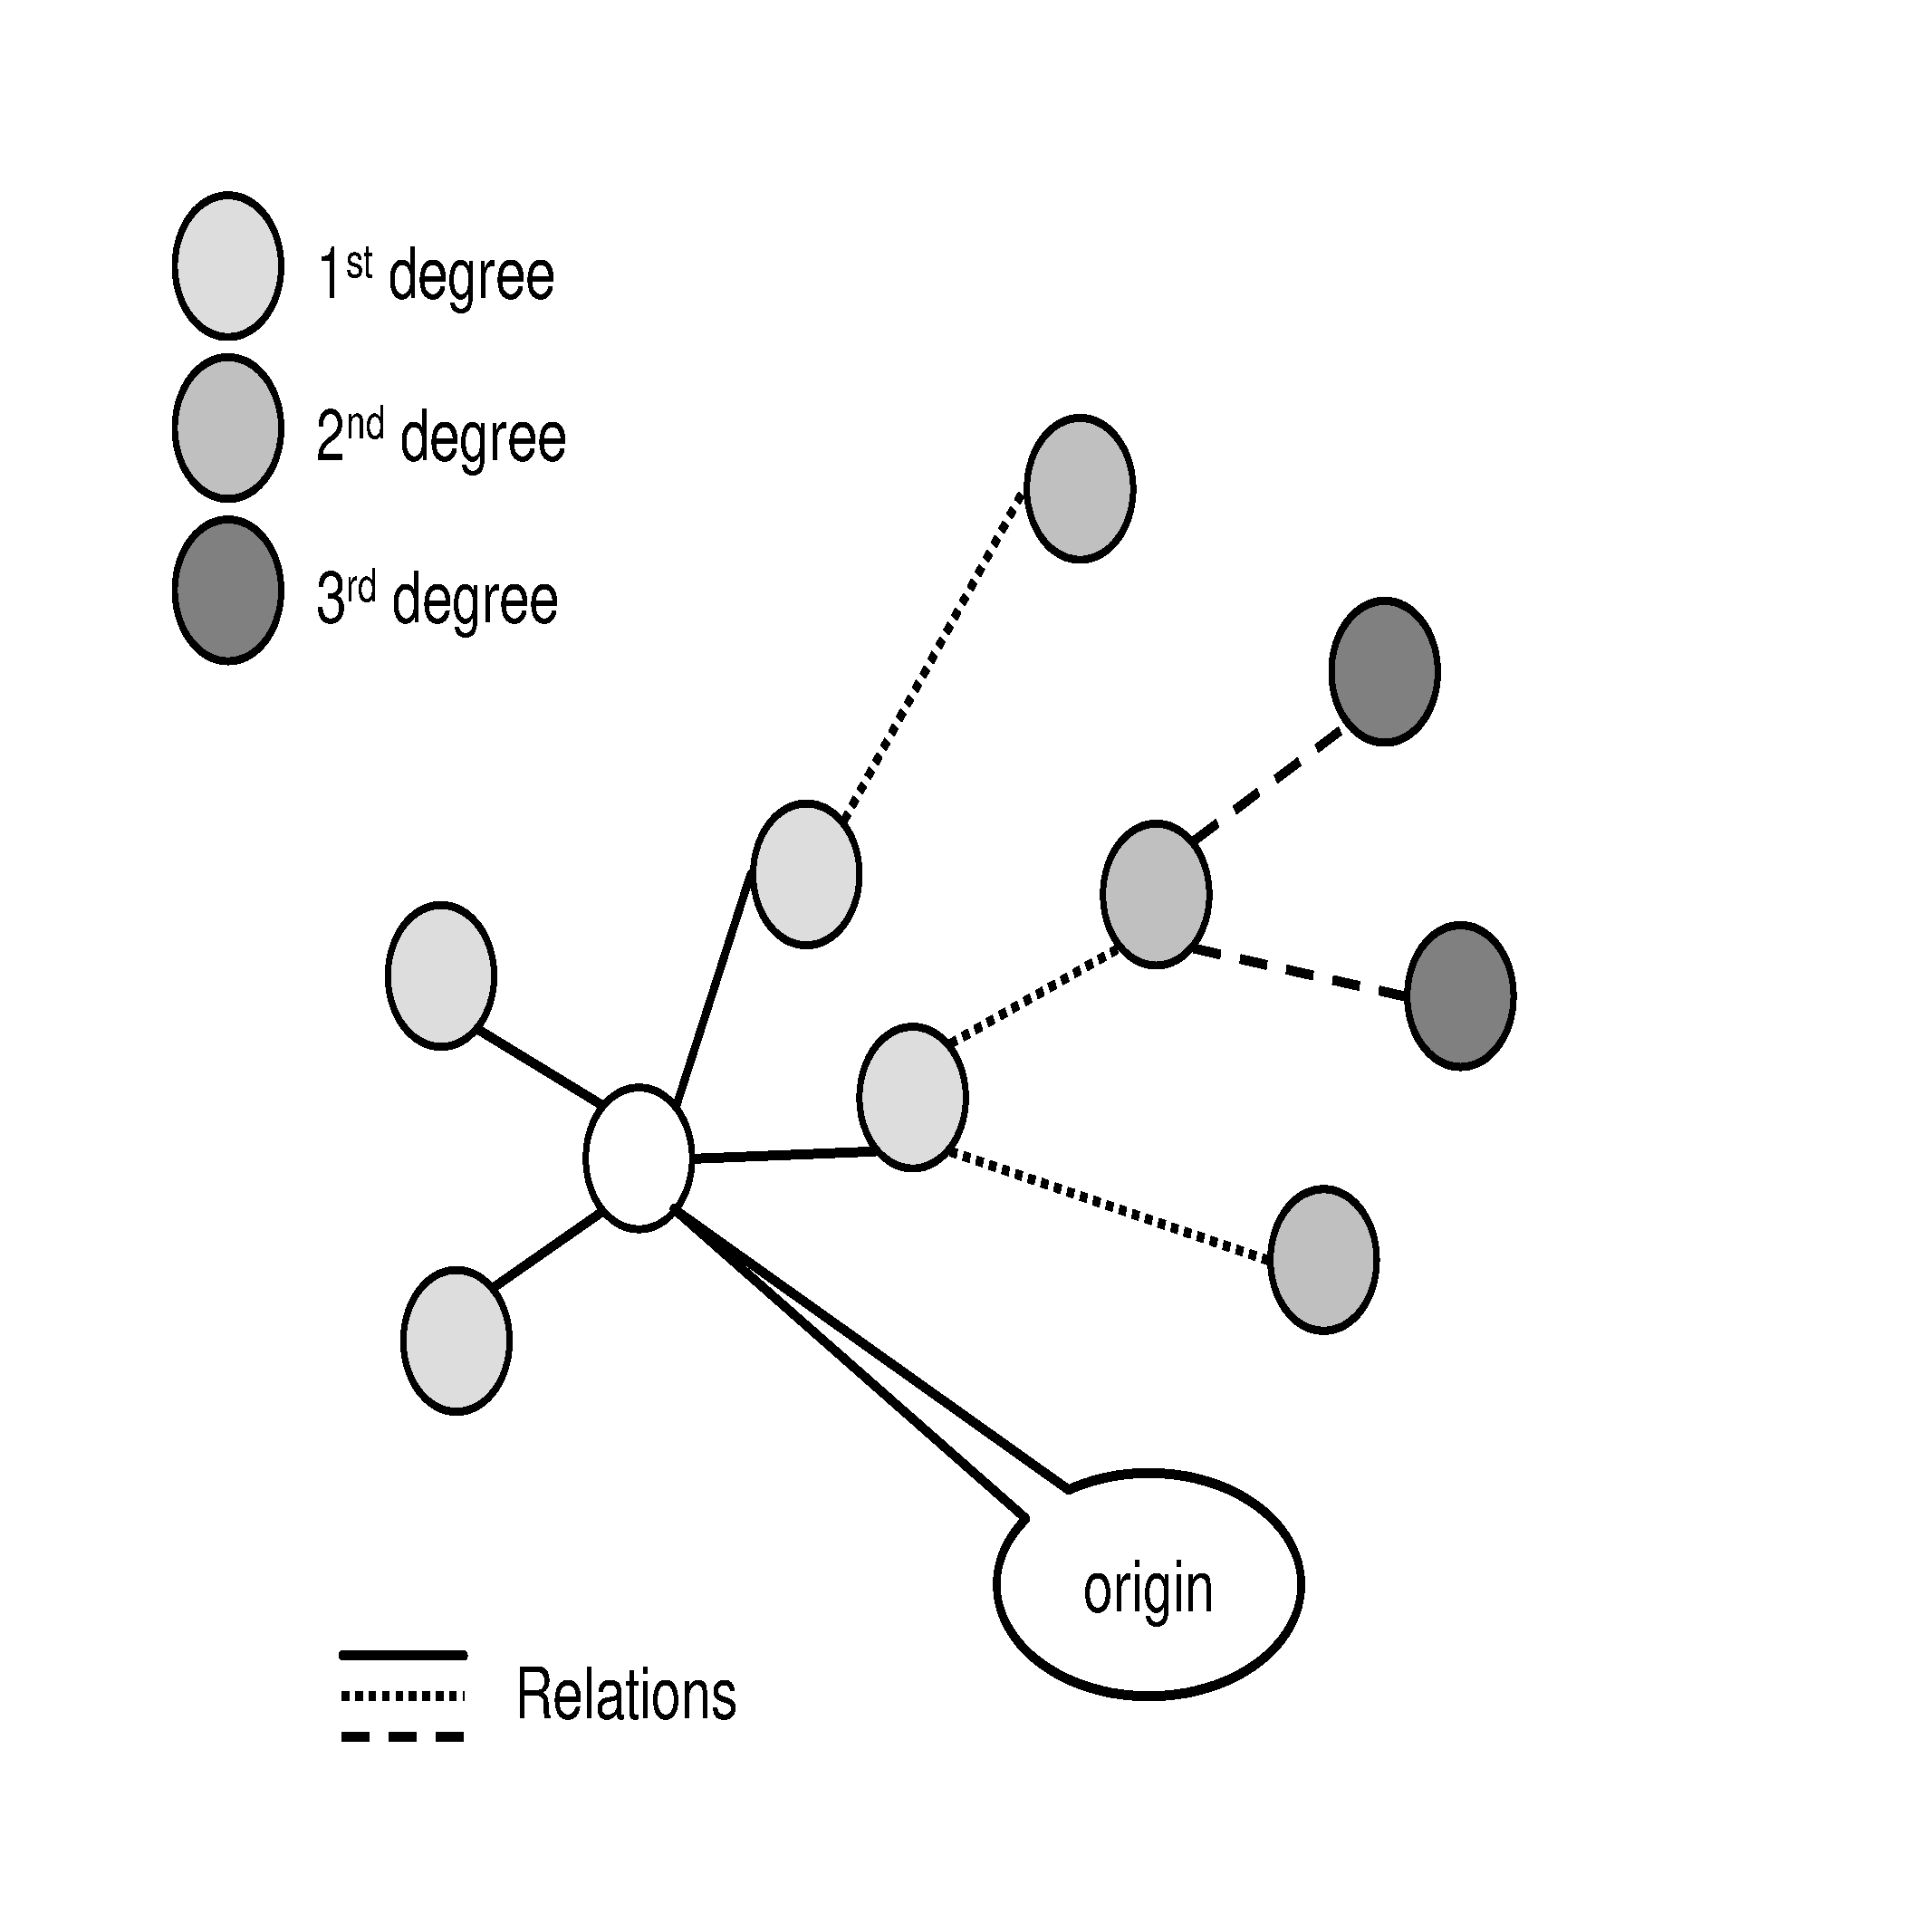
\includegraphics[width=10cm]{degrees}
	 \caption{Degrees of Relationship}
	 \label{degrees}
       \end{figure}
       The flexible setup of the relation finders means that the resulting 
       URLs may have different \textit{degrees} of relationship to the start 
       URL. 
       \begin{definition}
       If two URLs $ u_a $ and $ u_b $ are directly related by any given
       relationship $ \bullet $ (i.e. if $ u_a \bullet u_b $), 
       we call them related in the first degree.\\
       Some URL $ u_c $ is called related in the $ n^{th} $ degree to $ u_a $ if
       has no relationship with $ u_a $  but is related to an URL that 
       has a relationship of the degree $ (n-1) $ with $ u_a $. (e.g. if 
       $ u_a \bullet u_b$ and $ u_b \odot u_c $, then $ u_a $ and $ u_c $ are
       related in the second degree)
       \end{definition}
       The degree of relationship is the same as the length of a path between 
       two nodes in the graph model, and is an intuitive metric of how 
       \lq\lq far\rq\rq\ one web place is from another. Since this value is very 
       useful during processing the relation finders will mark all URLs with the 
       degree of relationship they have towards the original starting place.
     \subsection{Search Engines and Relation Finding}
       \begin{figure}[ht]
         \centering
         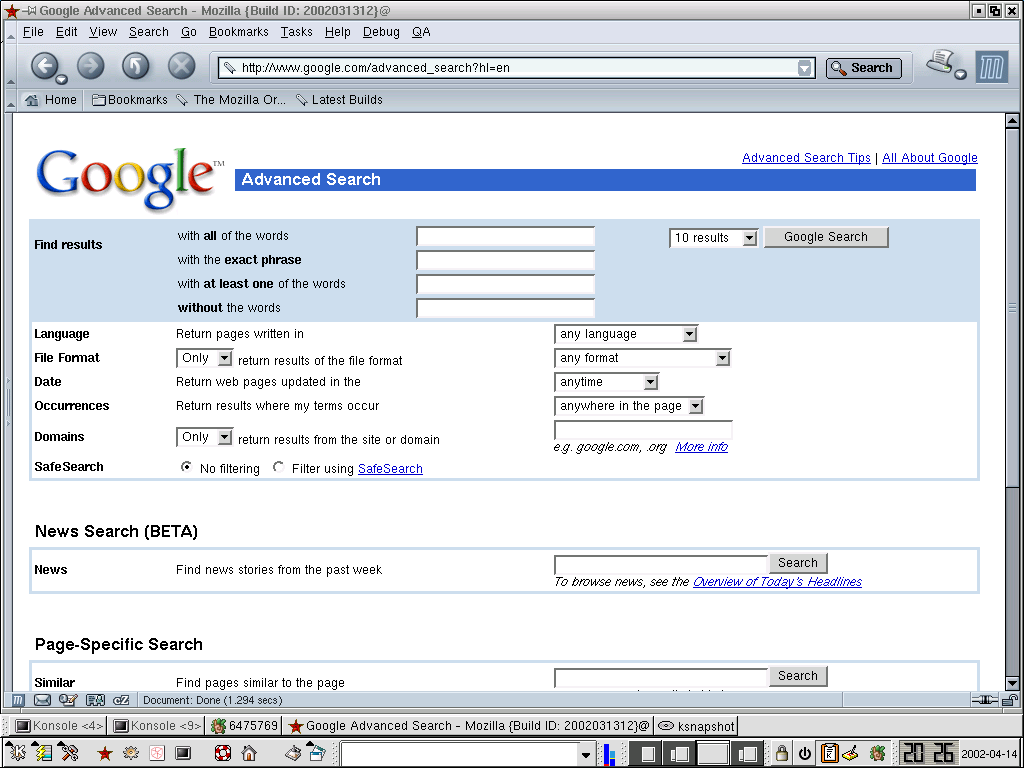
\includegraphics[width=10cm]{googleadv}
         \caption{Google Search Engine}
         \label{googleadv}
       \end{figure}
       Commercial web search engines like \cite{google} or \cite{altavista} have 
       some properties that make them well-suited for finding related URLs: They 
       use sophisticated web crawling and indexing techniques to build a 
       comprehensive index of the web, which can then be queried efficiently in 
       a multitude of ways. Usually the engines not only allow simple keyword 
       searches but allows empower the user to restrict the results to certain 
       languages, resource types or domain names. Some, like Google\cite{google} 
       even maintain the notion of related pages themselves, in features like 
       \lq\lq Find related pages\rq\rq\ or \lq\lq Find similiar\rq\rq . 
  
       Search engines will also use sophisticated ranking techniques, and 
       although the search engine rankings may or may not be useful in the 
       DoorStep ranking phase, they can always be used to select the best 
       possible candidates for the relation finding heuristic.
       
       Although the algorithms and techniques used within commercial search 
       engines are usually classified as trade secrets, it can be fairly assumed 
       that new research results are quickly adopted, due to the strong 
       competition between the different companies.
       
       The main drawback of commercial search engines (besides the \lq\lq black 
       box\rq\rq design) is that they are, well, commercial. Usually theses 
       engines may only be used freely for personal, interactive requests. An 
       example for these conditions are Google's terms of use\cite{googletou}:
       \begin{center}
       \begin{minipage}{10cm}
       \itshape
       [...] You may not take the
       results from a Google search and reformat and display them, or mirror
       the Google home page or results pages on your Web site. You may not
       "meta-search" Google. If you want to make commercial use of the Google
       Search Services, 
       [...]
       You may not send automated queries of any sort to Google's system
       without express permission in advance from Google. Note that 
       \lq\lq sending
       automated queries\rq\rq\ includes, among other things:
       \begin{itemize}
       \item{using any software which sends queries to Google to determine how
             a website or webpage \lq\lq ranks\rq\rq\ on Google for various 
             queries;}
       \item{\lq\lq meta-searching\rq\rq\ Google; and}
       \item{performing \lq\lq offline\rq\rq\ searches on Google.}
       \end{itemize}
       Please do not write to Google to request permission to 
       \lq\lq meta-search\rq\rq\
       Google for a research project, as such requests will not be granted.
       \end{minipage}
       \end{center}
       This means that publicly available DoorStep system will have to license 
       the use of the search engine or find a free one if it does not want to 
       build it's own web index (which is very demanding).
     \subsection{Rating function}
       Once a set of related URLs is found, one or more 
       \textit{rating functions} will be applied to the URLs. The goal
       of this step is to identify those web places which are the
       most interesting to the user. The concept of \lq\lq interesting to the
       user\rq\rq\ is rather hard to grasp algorithmically, so we will simply 
       say that a URL (or web place) is
       interesting in some aspect $ a $ if it certain properties that can be
       measured through a corresponding \textit{rating function} 
       $ f_a $. The rating of an URL $ u $ regarding this aspect
       can then be expressed as $ 0 \leq f_a(u) \leq 1 $.
       Examples of rating
       functions could be \lq\lq The resource does contain the specified
       keywords\rq\rq\ or \lq\lq The resource contains a text in the user's
       native language\rq\rq .
       
       The system may contain any number of rating functions $ f_1
       \dots f_n $ that measure different aspects that are of interest to
       the user.
       Each of these functions has a weight
       $ 0 < \alpha_i \leq 1 $ which indicates the importance of the given 
       aspect.
       The \textit{overall rating} $ \iota $ of an URL then calculates
       to:
       \[
         \iota(u) = \sum_{i = 0}^{n} 
	 \frac{\alpha_i f_i(u)}{n}
       \]
       An rating value of 1 indicates a most interesting web place
       while a
       value of 0 denotes a very uninteresting one. 
     \subsection{Filtering}
       The system allows for filters to be inserted between the different
       processing steps. A filter will typically check if an URL matches a
       predefined condition and discard it if it doesn't.
       
       Filtering can be used to remove \lq\lq noise\rq\rq\ from the input, to 
       speed up processing and also to remove the problem of 
       \lq\lq circular visit\rq\rq : When DoorStep systems are universally 
       employed, requests from one system would be registered as visits by 
       another system and the DoorStep systems would start visiting each other. 
       This can be avoided when the DoorStep system uses an unique 
       \verb$User-Agent:$ string and all visits by that agent are filtered out 
       before the processing starts.
  \section{Examples of relations}
    This section will, rather than trying to do an in-depth analysis, give some 
    comprehensive examples of relations between web places and explore their 
    possible meaning. We expected that most of the relations used in the 
    DoorStep system will be taken from independent research and that the quality 
    of such relations will be extensively analyzed in papers like \cite{links}.
    \\
    
    \textbf{Relation by hyperlinks:} These are probably the best understood and 
    most researched of all relations. Hyperlinks have several properties that 
    make them interesting to use in the DoorStep system: Hyperlinks are usually 
    set by people (rather than machines) and therefore denote social rather than 
    technical relations between web places. Adamic and Adar showed that 
    social groups can be identified by analyzing groups of hyperlinked web 
    pages\cite{links}. Hyperlinks are also very easily handle; no additional 
    information is 
    needed to follow a hyperlink to another web page and thus the respective 
    relation finder does not need a complicated heuristic.
    \\
    
    \textbf{Relation by domain:} DNS (sub-)domains usually denote geographic or 
    organizational groups. These can be very broad like the \verb$.com$ top 
    level domain, or quite specific like the \verb$computing.lancs.ac.uk$ domain 
    which contains the machines of the Lancaster University's computing 
    department. Finding web places within the same domain is not as 
    straightforward as following hyperlinks, the heuristic currently employed 
    in the DoorStep system is to query a commercial search engine for certain 
    keywords and restrict the search to a specific domain. This method also 
    ensures that the pages found by the relation finder are likely to be 
    interesting to the end user.
    \\
    
    \textbf{Relation by language:} Web places serving resource in the same 
    language usually come from the same (albeit very broad) cultural background. 
    For example, a page in Japanese language is usually written by a Japanese 
    person. Additional, the user of the DoorStep system may only understand 
    documents in certain languages and it may not be sensible to present him web 
    places that he cannot comprehend. The heuristic used for finding places with 
    a common language is the same as for finding pages in the same domain: Many 
    search engines allow to restrict the search to pages of a specific language.
    \\
    
    \textbf{Relation by referring search query:} As explained above, the 
    contents of the \verb$Referer:$ header (if existent) are retained within the 
    starting URL found in the first step. When a visitor was refered by a search 
    engine, the \verb$Referer:$ header will usually not only contain the 
    engine's URL, but the complete query string. This information allows a 
    relation finder to reproduce the search query and find out what other web 
    place (except our own) were returned by it. These places are related to the 
    starting URL in the way that \textit{a visitor from or near this place was 
    potentially interested in them} and they are related to our own place in the 
    way that they show up in the result of the same search query.
    \\
    
    \textbf{Relations from search engines:} Web search engines often maintain 
    their own notion of \lq\lq related\rq\rq\ pages, like Google's 
    \lq\lq Find related\rq\rq\ feature. While the exact definition of those 
    relations is hidden within the search engine a relation finder can very 
    easily exploit them -- simply by querying the search engine.
    \\
    
    \textbf{Relation by similiar hostname:} Some researchers (like 
    \cite[Link Affiliation]{experts}) 
    treat web places with similiar host names as related. For example they 
    assume that hostnames with the same prefix (like \verb$www.apple.com$ and
    \verb$www.apple.co.uk$) belong to the same organization. A heuristic for 
    finding this kind of relation could be somewhat more complicated since most 
    commercial search engines lack these kind of query options.
    \\
    
    For those heuristics that employ the use of search engines, it is important 
    to carefully select the search keywords. While the simplest method is to use 
    a set of static keywords which are deemed to be interesting to the user, 
    more sophisticated algorithms could also select new keywords from the web 
    places that have already been found.
  \section{Examples of rating functions}
    There is a lot of research on rating functions, and many different 
    approaches have been published, like PageRank\cite{page}, 
    Topic Destillation\cite{kleinberg} or
    anchor-text analysis\cite{chakrabarti}. 
    Although rating functions from 
    the literature may perform well, they are usually also quite complex and 
    require a lot of processing. Many, like the popular Link 
    Rating\cite{page}\cite{kleinberg}
    even require a more or less complete web index, something that is difficult 
    to build and maintain outside a lab enviroment. For this reason we will not 
    discuss those functions here, and instead present some simpler, home-grown 
    functions that are easy to implement and still perform reasonably well 
    within the DoorStep system. Nonetheless, it is always possible to enhance 
    the system with some more advanced rating functions if desired.
  
    \textbf{Keywords matching META tags:} This function can be used if the
    resource served by an URL is a HTML document containing tags of the form
    \verb$<meta name="keywords" content="keyword1,keyword2,..." />$ 
    We assume that the users interest is expressed in a list of $ n $ keywords,
    and for each occurrence of one of those keywords in the page's \verb$meta$
    keyword list $ KL $ the rating will be increased by $ 1/n $. Thus
    the rating will be:
    \[
      f_{\mbox{meta}}(u) = \sum{k_i \in KL_u} \frac{1}{n}
    \]
    \\
    
    \textbf{Keywords matching document body:} Especially if the page does not
    contain any \verb$meta$ tags we can try to find the keywords in the
    document's body. Since a word may occur in a page multiple times, we should
    also take the number of occurrences in account. ($ n(k_i) $ is the number of
    occurrences of the keyword $ k_i $).
    
    We will use a weight function $ w $ that assigns a weight to the occurrences
    of each keyword so that $ 0 \leq w(n(k_i)) \leq 1 $ and calculate the
    rating of the URL to
    \[
      f_{\mbox{key}}(u) = \sum_{k_i \in u} \frac{w(n(k_i))}{n}
    \]
    In the testbed implementation we then used a logarithmical function for 
    $w()$ that will quickly increase with the first few occurences of a 
    keyword but raise the rating more slowly if a huge number of occurences is 
    involved:
    \[
      - \frac{1}{log((n - \alpha) \beta) + 1}
    \]
    It showed that for most pages this method worked well, and with well-chosen 
    keywords and could distiguish pages that only dealt with the topic 
    marginally (like researcher's personal home pages) with those that covered 
    it extensively (like conference home pages).
    \\
    
    \textbf{Language or Domain match:} When one assumes that pages in a specific 
    language, within a specific domain or with some other static property or 
    more interesting to the user than others, a rating function can assign a 
    fixed rating to those pages.
    \\
    
    \textbf{Use search engine rating:} Most commercial search engines employ a 
    number of advance rating techniques, since it is the rating that really 
    distinguishes a good engine from a bad one. Although those mechanisms are 
    usually kept secret and cannot be accessed directly they are reflected in 
    the result of the search query. A rating function can exploit this property 
    and assign a higher rating to pages that show up at the top of the search 
    results than to those on the bottom.
  \section{Test Implementation}
    \subsection{Testbed Architecture}
      In order to evaluate our assumptions, we implemented a testbed that 
      allowed us to test the DoorStep system in a real-life enviroment, using 
      the relations and rating functions given in the examples sections (FIXME: 
      Refer to sections).
      
      The testbed consists of a collection of modules, exchanging XML formatted 
      data: There is one XML format to describe generic \textit{visit events} 
      (Figure \ref{visitxml}) while another is used to describe \textit{web 
      places} (i.e. URLs, Figure \ref{urlxml}). Each module will read XML 
      documents of one of those formats and will produce a document in the URL 
      description format as an output.
      
      \begin{figure}[ht]
\begin{verbatim}
<visitlist>
  <visit>
    <type>Html</type>
    <timestamp>01:11:2001:00:00:42</timestamp>
    <visitor>
      <class>remote</class>
      <class>agent</class>
    </visitor>
    <resource>/lehre/ubiq/kontext/html/tsld010.htm</resource>
    <host>dudley.waltham.northernlight.com</host>
    <location_code>244</location_code>
  </visit>
  <!-- The file may contain more visits -->
</visitlist>
\end{verbatim}
        \caption{XML format for visits}
	\label{visitxml}
      \end{figure}
      \begin{figure}[ht]
\begin{verbatim}
<url_list>
<url>
  <name>http://dudley.waltham.northernlight.com/</name>
  <location_code>244</location_code>
  <timestamp>01:11:2001:00:00:42</timestamp>
  <degree>0</degree>
  <interest>0.5344394</interest>
  </url>
  <!-- The file may contain more URLs -->
</url_list>
\end{verbatim}
        \caption{XML format for URLs (web places)}
	\label{urlxml}
      \end{figure}
      
      The modules will be arranged in a daisy-chain, with a visit-to-url module 
      (called an \textit{extractor} at the head of the chain and any number of 
      url-to-url modules (called \textit{refiners}) following. The contract of 
      an extractor module requires that it finds URLs close to the visits given 
      in the input document (thus performing the first step in the DoorStep 
      processing chain). The \textit{extractor's} output is expected to be a 
      document describing those URLs. The contract of a \textit{refiner} module 
      requires that it acts either as a \textit{relation finder} or a 
      \textit{rating function}. If the \textit{refiner} acts as a rating 
      function it is expected to assign a rating value to each of the URLs on 
      the input. If an URL already has a rating, it shall be modified according 
      to the \textit{refiner's} internal weight. A \textit{refiner} acting as a 
      \textit{relation} finder is expected to read the URLs from the input 
      document and find other places related to them (by a relation that is 
      configured within the \textit{refiner} module).
      
      A \textit{refiner} acting as a \textit{relation finder} can be configured 
      with a maximum degree of relationship. If a URL is encountered with a 
      higher degree of relationship the refiner shall \textbf{not} attempt to 
      find URLs that are related to it -- the URL must be passed on to the 
      output unmodified. This property allows to mimick the flexible setup as in 
      figure \ref{relations} while the \textit{relation finders} are only 
      connected in a simple daisy-chain. (\textit{Refiners} acting as rating 
      functions must ignore the degrees of relationship). It is also required 
      that rating functions must be on the end of the chain.
      
      FIXME:GRAPHIC
      
      Each module in the system can contain one or more filters. A filter may 
      remove any entity (visit or URL) from the input \textit{before} any 
      processing is done. The entity will permanently be removed from all 
      processing.
    \subsection{Test Framework}
      For practical reasons we created a framework of Java classes that 
      implements the basic functionality of the \textit{extractors} and 
      \textit{refiners}, is capable of handling the connections between the 
      modules and takes care of recurring tasks (e.g. XML decoding or search 
      engine requests). Due to the framework a new module type can (in many 
      cases) be implemented by overwriting but a single method of the 
      framework's superclass.
      
      Nevertheless it is not required that each module is part of the 
      framework or even written in Java at all. As long as a module is able to 
      understand the respective XML format(s) and conforms to the contracts 
      given in the previous section it should be able to interact with all 
      other modules.
    \subsection{User Display}
      The testbed also contains a display architecture that shows a \lq\lq slide
      show\rq\rq of the resulting web pages. The architecture consists of a
      Java-driven web application using servlets and JSPs and requires only a
      standard web browser as a front end. Alternatively, the Display may run a
      small VisualBasic application that is directly driven by a Java server
      process and offers some additional functionality.
      
      The display is meant to run on a separate screen in the user's enviroment
      and change infrequently (i.e. every 2 to 10 minutes) to a new web place.
      If the user is interested in a certain page he has the option to stop the
      slide show and explore that page further (by following the hyperlinks on
      the page). The slide show will automatically commence after a while.
      \begin{figure}[ht]
       \centering
	 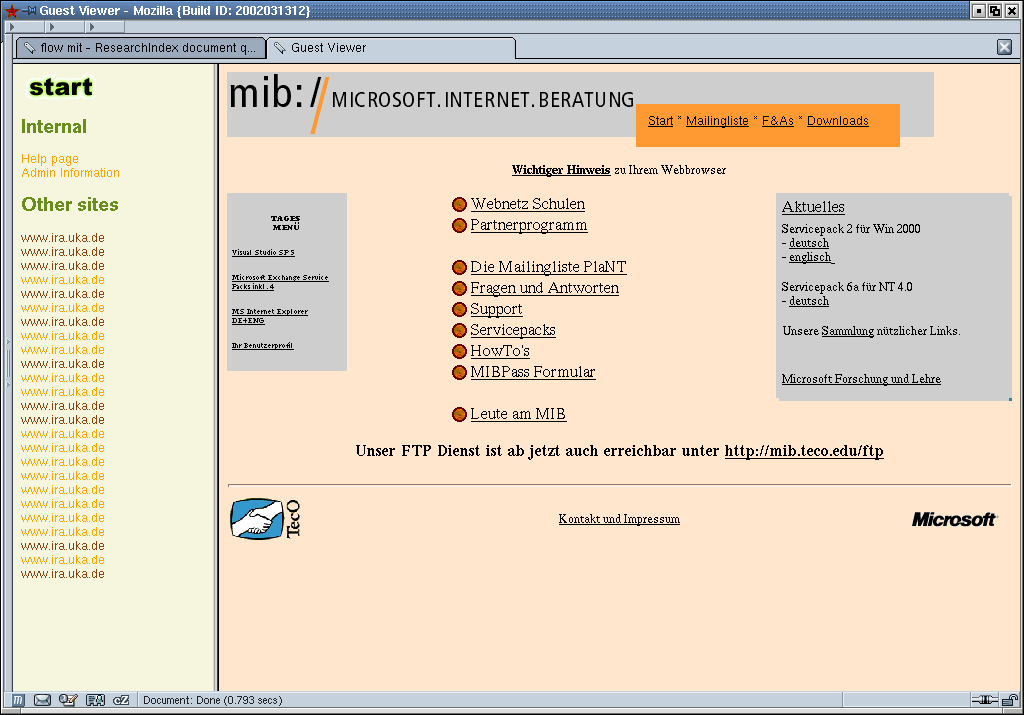
\includegraphics[width=10cm]{javaclient}
	 \caption{Java Based Display}
	 \label{javaclient}
       \end{figure}
      
      For a first user study we plan to use this software on a panel computer 
      that can easily be fitted in the user's surroundings. The machine is 
      equipped with a touch-sensitive panel for intuitive user interaction and 
      should easily blend into any office enviroment. This kind of ambient 
      display should be unobtrusive to the user while at the same time enabling 
      him to check his web surroundings whenever he chooses to.
      (FIXME:Screenshots,Picture)
    \subsection{Walk-Trough Scenario}
      In this small scenario we will follow the way that three visit events take 
      through the system. We will see how the visits are handled and how related 
      web places are found. Our example system will be set up in the following 
      way (line numbers given for reference only):
      \begin{verbatim}
010 extractor = new ExtractingChain(dataSource);
020 String keywords = "wearable,ubicomp";
030  
040 Extractor ext = new StraightExtractor();
050 ext.addPrefilter(new LocalVisitFilter());
060 ext.addPrefilter(new AgentVisitFilter());
070 extractor.setExtractor(ext);
080        
090 SearchingRefiner search = new SearchingRefiner();
100 search.setKeywords(keywords);
110 extractor.addRefiner(search);
120        
130 extractor.addRefiner(new LinkRefiner());
140                
150 KWInterestRefiner kwr = new KWInterestRefiner(); 
160 kwr.setKeywords(keywords); 
170 extractor.addRefiner(mkr); 
        \end{verbatim} 
        The \verb$ExtractingChain$ in line 10 is an utility object that will 
        connect the Extractor and several refiners. The \verb$StraightExtractor$ 
        in line 40 implements the algorithm introduced in section FIXME:REF, and 
        it's prefilters (lines 50 and 60) will discard visits that come from the 
        local network, or any automated web agent.
        
        The \verb$SearchingRefiner$ in line 90 will search for URLs in the same 
        domain as the starting point and the \verb$LinkRefiner$ (line 130) will 
        follow hyperlinks.
        
        Finally, the \verb$KWInterestRefiner$ in Line 150 will use the rating 
        function introduced in FIXME:REF to rate the URLs.
  \section{Test System Performance} 
    Although a formal user study has yet to be planned, we did 
    preliminary tests on the system in two ways: First we installed the JSP 
    server on a machine available to the research group, and fed it with the 
    log data from our own web server (at 
    \textit{http://ubicomp.lancs.ac.uk/). This allowed us not only to test 
    the long-term stability of the software, but also to observe if and how 
    the system would be used. In many cases we were quite surprised about 
    the web places found by the system, and most of them were related to our 
    research. The main problem with the test setup was that the traffic on 
    our own machine is quite low, allowing the system to find new places 
    only very infrequently. Researchers that did not have their own display 
    for the DoorStep system did not use it permanently, but rather looked 
    the page up during their spare time.
    
    For the second test we performed some offline processing on a large log 
    file, in order to get some statistical results. This test will be explained 
    in detail in the next sections.
    \subsection{Test Data}
      The test dataset is part of the HTTP log file from a research lab
      web server. The log file contains about 200.000 entries from a period of
      about 2 weeks.
      
      The file contains a high amount of redundancy and noise: The 200.000 
      entries record visits from only 5720 different clients. Of those, 1603 
      were either visits from local clients (within the same network as the 
      server), failed to retrieve a resource or were requests for pictures 
      within sites.
      
      Most of the remaining entries (82\%) came from a machines with a proper
      DNS host name, and only 18\% from unresolveable addresses -- this indicates
      that methods requiring qualified DNS names should work reasonably well. A
      substantial amount of the entries also carried additional information:
      Almost 40\% of the requests were made by automated agents (e.g. web
      crawlers) that idendentifiable by an \verb$User-Agent$ String and 8\% of
      were referred to the site as the result of a web search (with the search
      string showing up in the \verb$Referer$ field). (FIXME:Update numbers 
      here)
    \subsection{Results}
      For the trials we used an \textit{extractor} module implementing the
      metric defined in (FIXME:Reference) to find living URLs, an
      \textit{refiner} module searching the original URLs domain for certain
      keywords and one following the hyperlinks of the original URL. The results
      were rated by two \textit{refiner} modules implementing the rating
      functions given in (FIXME:Reference). The input to the system consisted of
      the 3500 unique and sucessful visits from the original log.
      
      Out of these, the \textit{extractor} module found about 1500 URLs that
      were \textit{alive}. This is a reasonably good set of starting places,
      however a first look at the data revealed that most of them were either
      ISP portal pages or homepages of academic institutions. While the latter
      are in most cases good starting points for further processing, ISP portal
      are rather unspecific and uninteresting in the context of this system.
      This behaviour is mostly due to the fact that many of the \lq\lq
      mundane\rq\rq\ (i.e. non-academic) visitors are \lq\lq homeless\rq\rq\ in
      the sense that the do not have their own web place -- and even if they do
      they often enter the web from a place that is far removed from their own
      place. In a purely academic setting (like ours) this problem is less
      pressing since the user's home place (or -page) is usually loacted within
      the same network from which the user enters the web. This \lq\lq homeless
      visitor problem\rq\rq\ has already been observed in \cite{webaware}, and 
      some; this will be an issue for further research.
      
      (FIXME:Refiner Results)
      
      We observed that the rating functions worked quite well under most 
      circumstances: When using keywords from our research area (like ubicomp, 
      wearable or context), directly research-related pages (like conference 
      home pages) would usually rank quite high, completely unrelated pages 
      ranked zero. Indirectly related pages (e.g. researchers' web pages)
      get a medium rating. Pages found by the web search based relation finders 
      always rank well, since the the rating functions use the same keywords. We 
      also found that places related to well-rated URLs 
      * Will they also rank well?
  \section{Privacy: Reassuring the Visitors}
    A system that, like DoorStep, collects and analyzes user data most always 
    take privacy considerations into account. 
    
    In practice, usage data falls into two broad categories: Statistical usage 
    data which cannot be linked to any particular user, and is therefore less 
    confidential, and personal data which can identify the 
    person to which the data \lq\lq belongs\rq\rq . The personal data is 
    sometimes further divided according to confidentiality: While the address or 
    phone number of a person is usually publicly known, medical records should 
    be kept strictly confidential. It is generally agreed that it is the 
    responsibility of the operator of any data processing service to safeguard 
    sensitive personal data, although not always on the methods with which this 
    can be achieved. 
    
    Due to technical and legal requirements, a lot of sensitive personal 
    information is stored within web server log files. Each request will be 
    logged on all machines along it's way, and if this log information is 
    combined it is not only possible to link each page view to a particular 
    person but also to create a profile of that person's behaviour on the web. 
    And although the extent of the logging is by no means a secret, the majority 
    of web users is not aware of it, still thinking they are anonymous; even 
    those who are aware of the logging are under the impression that the logs 
    will probably never be read.
    
    Since the web server log files contain highly sensitive data, their use is 
    regulated by tight regulations in many parts of the world. Despite the fact 
    that some countries (like the USA) leave privacy considerations largely to 
    the forces of the market, others have imposed a rather strict legislation: 
    In Germany, for example, even if the log data has been collected legally, it 
    still be illegal to use it for purposes the visitor has not agreed to, or 
    the data is anonymized.
    
    The DoorStep system may still be safely employed in those countries, since 
    it treats the log data as anonymous and does not present any personal data 
    to the user (the web pages that are displayed by the system can hardly be 
    regarded as confidential information). Nevertheless, care should be taking 
    in employing such systems: Not only is IT law often a doggy ground, but an 
    improper application of the system may also damage reputation of the 
    operator: Even though most users are quite oblivious of privacy 
    considerations in areas they fell \lq\lq safe\rq\rq\ in, they often are very 
    careful about new developments (e.g. student's comments about the current 
    project ranged from \lq\lq doggy ground\rq\rq\ to \lq\lq Big Brother\rq\rq 
    ).
    
    Engineers are often surprisingly aware of the privacy implications of their 
    inventions, and many specification documents warn against the abuse of 
    certain features -- like, for example, the HTTP specification\cite{http}:
    
    FIXME:QUOTE
    
    If the DoorStep (or a similiar) system sees widespread use, the safest and 
    most honest thing to do is to include some option into the visitors user 
    agent to disable the DoorStep processing, and the user agent would then 
    signal DoorStep to ignore the visit.
  \section{Conclusions and Further Work} In this work we showed that, using 
    the notion of \textit{relations} between web places, it is possible to build 
    a system that can help to visualize the connections between a site and the 
    visitors. The system should renew the hosts' interest in maintaing his own 
    web place and, by allowing a look into the virtual surroundings, give new 
    incentives for improvements. The test installation has been well recieved 
    within the group, and the results were interesting and suprising. On one 
    occation a researcher even messaged us if we could \lq\lq wind back\rq\rq\ 
    the slide show to an interesting page that he saw -- this feature will be 
    implemented in a future version.
    
    For interested users we will also keep a public DoorStep web server running
    so that everyone with a spare machine will be able to use the system.
    
    Intial user reactions within the reasearch group were positive and we now
    plan to conduct a small user study that will allow us to study users
    reactions over the period of a few weeks. We hope to get an impression on how
    the use of the DoorStep system changes the host's attitude towards his own
    web place and which places he will be most interested in. The results of the
    user study will also go into the future development of the system.
    
    In the future we plan to make the DoorStep system more adaptive so that
    rather than relying on a fixed set of keywords it will learn the user's
    preferences and modify it's behaviour in different enviroments. We also need
    to fix the \lq\lq homeless visitor problem\rq\rq : The most permanent
    solution would be for the visitor to supply his own home URL \cite{webaware},
    through an additional HTTP header field, although this would require
    modifications to the visitor's client software. Other options would include
    to use information from existing profiling systems (FIXME:REFER TO SUCH) or
    information from user accounts.
  \begin{thebibliography}{99}
    \bibitem{awstats} AWStats Tool
    \bibitem{webaware} Hans-W. Gellersen and Albrecht Schmidt.
    Look who's visiting: supporting visitor awareness in the web.
    Academic Press, 2000.
    \bibitem{experts} Krishna Bharat and George A. Mihaila.
     When Experts Agree: Using Non-Affiliated Experts to Rank Popular Topics,
     Proceedings of the WWW10 Conference, 2001.
     http://www10.org
    \bibitem{flake} C. Flake, S. Lawrence and C. Lee Giles.
    Efficient identification of web communities.
    Sixth ACM SIGKDD Internation Conferenc on Knowledge Discovery and Data 
    Mining, Boston, MA, 2000. 
    pp. 150-160
    \bibitem{gibson} D. Gibson, J. Kleinberg and P. Raghavan.
    Inferring Web communities from link topology.
    Proceedings of the 9th ACM Conference on Hypertext and Hypermedia, 1998.
    \bibitem{links} Lada A. Adamic and Eytan Adar.
    Your are what you link, Proceedings of the WWW10 Conference, 2001.
    http://www10.org/program/yawyl/YouAreWhatYouLink.html
    \bibitem{page} S. Brin and L. Page.
    The anatomy of a large-scale hypertextual web search engine, 
    Proceedings of the WWW10 Conference, 2001.
    http://www10.org
    \bibitem{kleinberg} J. Kleinberg.
    Authoritative sources in a hyperlinked enviroment, Proceedings of the WWW10
    Conference, 2001.
    http://www10.org/
    \bibitem{chakrabarti} S. Chakrabarti, B. Dom et. al.
    Experiments in topic distillation.
    Proceedings of ACM SIGIR Workshop on Hypertext Information Retrieval on
    the Web, 1998.
    \bibitem{ambient} Hans-W. Gellersen, Albrecht Schmidt and Michael Beigl.
    Ambient Media for Peripherial Information Display.
    \bibitem{windows} Liechti O, Siefer N and Ichikawa T.
    A non-obtrusive User Interface for Increasing Social Awareness on the 
    World Wide Web. Personale Technologies 3 (1\&2), 1999.
    \bibitem{url} RFC 1738. Uniform Resource Locators (URL) 
    \bibitem{logfile} Log file RFC.
    \bibitem{google} Google URL: http://www.google.com/
    \bibitem{googletou} Google: Terms of Use
    \bibitem{http} HTTP RFC
    \bibitem{dns} RFC 1035. Domain Names - Implementation and Specification
  \end{thebibliography}
\end{document}
